\documentclass[../mcmpaper]{subfiles}
\begin{document}
\section{Model Estimating and Solving of Problem 1 }
\subsection{Data Preprocessing}
In order to analyze the travel characteristics of people in the city, we analyze the data given in the annex with different parameters such as travel time, payment method, payment proportion of different payment methods, hoping to summarize the travel payment characteristics.
\par
According to the data given in the table in Annex 1, we need to find out the relationship between travel payment method and travel time, so as to analyze the payment characteristics of passengers.
\par
\textbf{Step 1:}\space read in data-use pandas to read in the data in the given table.
\par
\textbf{Step 2:}\space column name modification - due to the different column names in the given table, we will modify the column name to a unified column name in order to make the subsequent data consolidation normal.
\par
\textbf{Step 3:}\space merge data-merge the data in 28 tables and sort them out.
\par
\textbf{Step 4:}\space remove abnormal data - in order to analyze the two payment methods between mobile payment and bus card payment, we will display null (no card swiping) and 0001-1-1 (no card swiping record, because of machine failure, but the card swiping method is still recorded.) which are not included in the calculation and output charts. 
\subsection{Data Analysis}
It can be seen from the data preprocessing stage that after the preliminary work , we use \textbf{pandas} to output visual charts and analyze the data according to the intuitive charts.

\begin{enumerate}[label=\arabic*., format=\bfseries, itemindent=0pt, leftmargin=0pt, topsep=0pt, listparindent=\parindent, itemsep=1pt]
    \item Divide the day into 24 hours as the abscissa, and accumulate the payment times of the two methods respectively. Set the orange line in the figure to represent the payment times of boarding with a bus card, and the blue line to represent the payment times of using a third-party mobile payment platform. The chart can be obtained, as shown in Figure~\ref{fig:5.1}.\\
% \begin{figure}[!ht]
% \centering
% 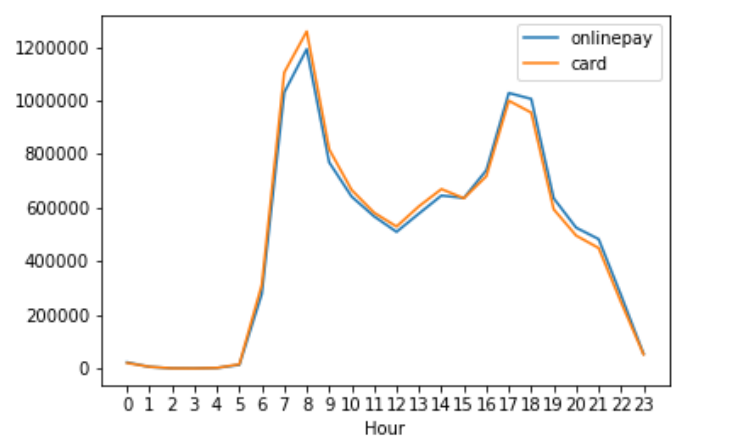
\includegraphics{5}
% \caption{The graph of the consumption times of the two payment methods changing with the hour}
% \label{fig:5.1}
% \end{figure}
\begin{minipage}{1.0\linewidth}
\centering
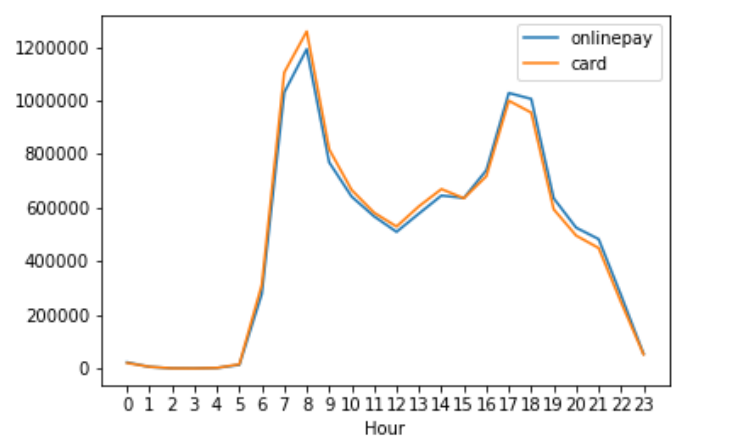
\includegraphics{5}
\captionof{figure}{The graph of the consumption times of the two payment methods changing with the hour}
\label{fig:5.1}
\end{minipage}
\par
During the period from 23:00 to 5:00 the next day when the bus and subway are not running, the data in the figure shows that from 5:00 to 7:00, the orange line almost coincides with the blue line, which means that the payment times paid by bus card and third-party mobile platform are almost the same. From 7:00 to 15:00, the orange line is slightly higher than the blue line, Between 7:00 and 8:00, the orange line is significantly higher than the blue line, which shows that the number of bus card payments is obviously more than the third-party payment platform. From 15:00 to 22:00, the blue line is slightly higher than the orange line. From 17:00 to 18:00, the blue line is significantly higher than the orange line, that is, the payment times of the third-party mobile payment platform are significantly higher than that of the bus card.
\par
The reason may be that many people who are not familiar with using the third-party payment platform (such as older elders) will choose to travel during this period during the morning rush hour, so the payment times of using the bus card will be more. The evening peak is mostly composed of young people after work and school, and they are more dependent on the third-party payment platform, so it will cause the lines in the diagram.
% \begin{figure}[!ht]
% \centering
% 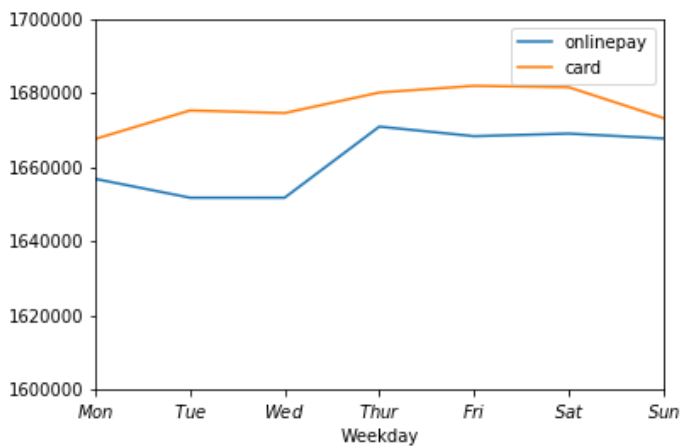
\includegraphics{6}
% \caption{The graph of the change of the consumption times of the two payment methods with the number of Sundays}
% \label{fig:5.2}
% \end{figure}
    \item Divide the given 28 day data into seven days from Monday to Sunday by week, and still add up the payment times. The orange line in the figure represents the payment times by using the bus card, and the blue line represents the payment times by using the third-party mobile payment platform. The broken line diagram is shown in Figure~\ref{fig:5.2}.\\
\begin{minipage}{1\linewidth}
\centering
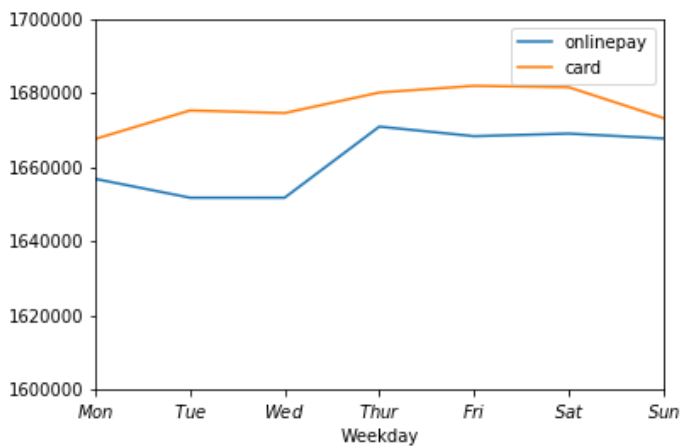
\includegraphics{6}
\captionof{figure}{The graph of the change of the consumption times of the two payment methods with the number of Sundays}
\label{fig:5.2}
\end{minipage}
\par
It can be seen from the broken line diagram that there is little difference between the number of people using bus cards and the third-party mobile payment platform (it should be noted here that in order to see the specific situation between the broken lines, we reduce the value interval of the whole vertical axis, but in fact, the difference between the two figures is still not large), However, generally speaking, the number of payments using the bus card is greater than that using the third-party mobile payment platform. It can be seen that the difference between the two is the largest on Wednesday and the smallest on Thursday and Sunday.
\par
Except for some errors in statistical data, the reason may be related to people's preference for travel choice. The number of people who travel on weekdays will peak on Thursday and then stabilize and begin to decrease on weekends. Since the promotion of third-party payment platforms may not be very popular, it can be seen that the number of payments using bus card is still slightly higher than that of mobile payment, but the difference between the two is very small.
% \begin{figure}[!ht]
%     \centering
%     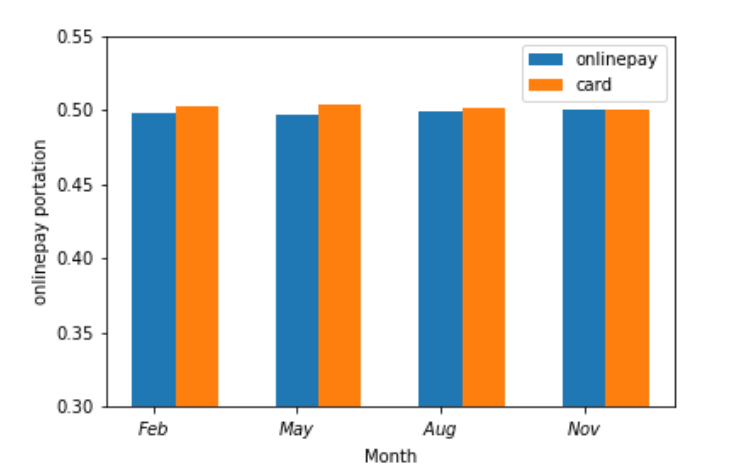
\includegraphics{7}
%     \caption{Bar chart of monthly proportion of consumption times of two payment methods}
%     \label{fig:5.3}
% \end{figure}
    \item The data given in Annex 1 are the data collected in February, may, August and November respectively. The abscissa is arranged by month, and the proportion of bus card payment and third-party mobile payment platform payment is taken as the abscissa. The calculated chart is shown in Figure~\ref{fig:5.3}.\\
\begin{minipage}{1.0\linewidth}
    \centering
    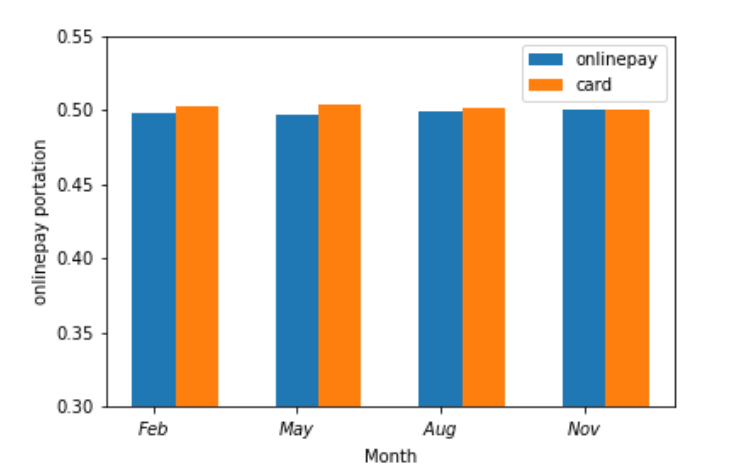
\includegraphics{7}
    \captionof{figure}{Bar chart of monthly proportion of consumption times of two payment methods}
    \label{fig:5.3}
\end{minipage}
\par
We can see from the figure that the gap between the two is very small, that is to say, the number of payments using bus cards is basically the same as that using third-party payments. We can see that the payment times of bus cards in February, may and August are less than those of third-party payment platforms. In November, the two reached balance. And it can be seen that with the increase of months, the number of payments on third-party payment mobile platforms is also increasing slightly.
\par
The main reason is that various cities across the country have promoted the use of mobile payment platforms since 2017, and the promotion work has been basically completed by the end of 2017. Therefore, with the passage of months, the number of payments using third-party payment platforms will increase accordingly. As reflected in the data chart, we can see that the proportion of third-party payment platforms is rising slowly.
% \begin{figure}[!ht]
% \centering
% 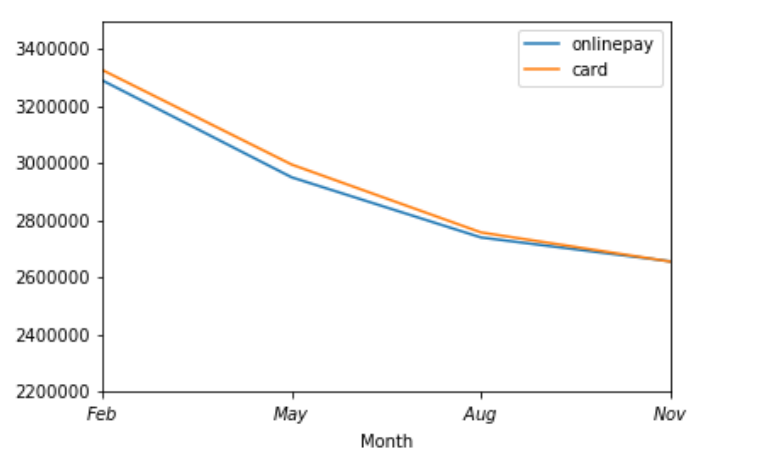
\includegraphics{8}
% \caption{The change of consumption times of two payment methods by month}
% \label{fig:5.4}
% \end{figure}
    \item According to the data given in Appendix 1, taking four months as the abscissa, we will sum up the payment times of the two methods. The orange line in the figure represents the payment times of getting on the bus with the bus card, and the blue line represents the payment times by using the third-party mobile payment platform. The two curves obtained from the payment times of the payment platform are shown in Figure~\ref{fig:5.4}.\\
\begin{minipage}{1.0\linewidth}
    \centering
    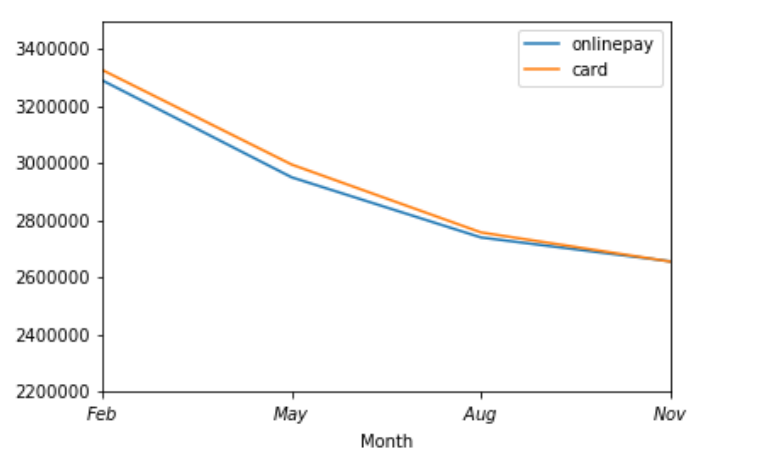
\includegraphics{8}
    \captionof{figure}{The change of consumption times of two payment methods by month}
    \label{fig:5.4}
\end{minipage}
\par
As shown by the curve in the figure, it can be seen that with the increase of months, the overall number of payments using both methods is decreasing, and the decreasing range is almost the same. At the same time, in the process of reduction, the number of payments using the bus card is always higher than that using the third-party mobile payment platform, until August and November, the two are almost equal.
\par
The reasons can be speculated as follows: 1 Due to statistical problems, the number of samples collected in the last three months was less than that in the previous few months.2 Since we excluded the options of not swiping and unsuccessful swiping at the beginning, it is also possible that the number of unsuccessful swiping is higher and higher as the month goes on, and the sample of statistical data will be less and less. III With the passage of months, the number of people who choose bus cards and third-party mobile payment platforms to pay gradually decreases, which may be due to the decrease in the number of people who choose to take buses or the increase in the number of cash payments.
\begin{figure}[!ht]
\centering
\begin{minipage}[c]{0.45\linewidth}
    \centering
    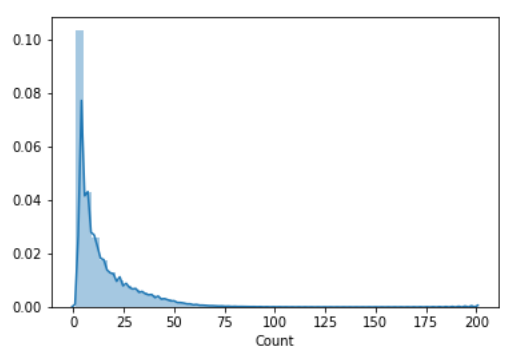
\includegraphics[scale=0.8]{9}
    \caption{User's 28-day travel times and distribution of users}
    \label{fig:5.5}
\end{minipage}
\qquad
\begin{minipage}[c]{0.45\linewidth}
    \centering
    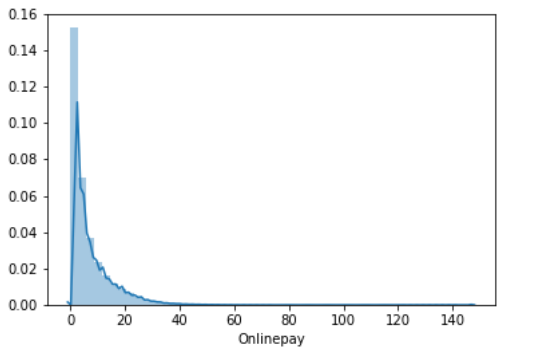
\includegraphics[scale=0.8]{10}
    \caption{User's 28-day travel mobile payment times and distribution}
    \label{fig:5.6}
    \end{minipage}
\begin{minipage}[c]{1\linewidth}
    \centering
    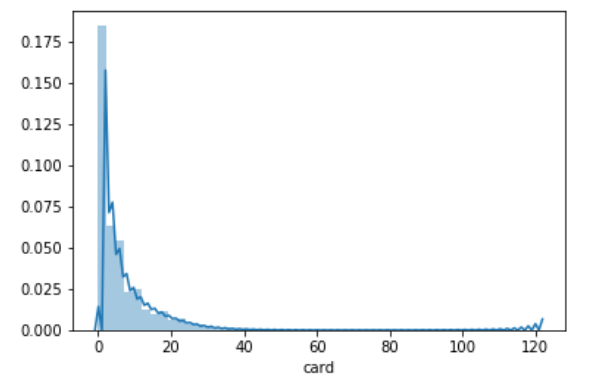
\includegraphics{11}
    \caption{User's 28-day bus card payment trip times and distribution map}
    \label{fig:5.7}
\end{minipage}
\end{figure}
% \begin{minipage}{1.0\linewidth}
% \begin{minipage}[c]{0.45\linewidth}
%     \centering
%     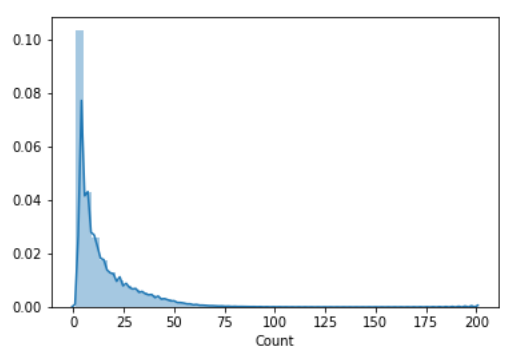
\includegraphics[scale=0.8]{9}
%     \captionof{figure}{User's 28-day travel times and distribution of users}
%     \label{fig:5.5}
% \end{minipage}
% \qquad
% \begin{minipage}[c]{0.45\linewidth}
%     \centering
%     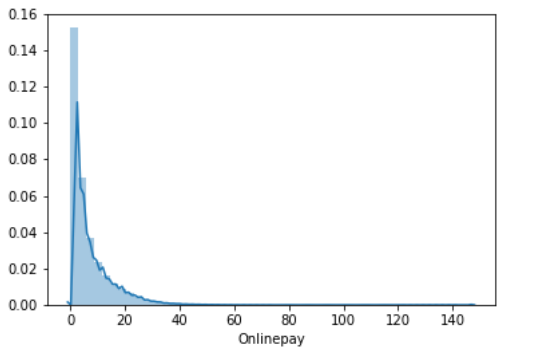
\includegraphics[scale=0.8]{10}
%     \captionof{figure}{User's 28-day travel mobile payment times and distribution}
%     \label{fig:5.6}
%     \end{minipage}
% \begin{minipage}[c]{1\linewidth}
%     \centering
%     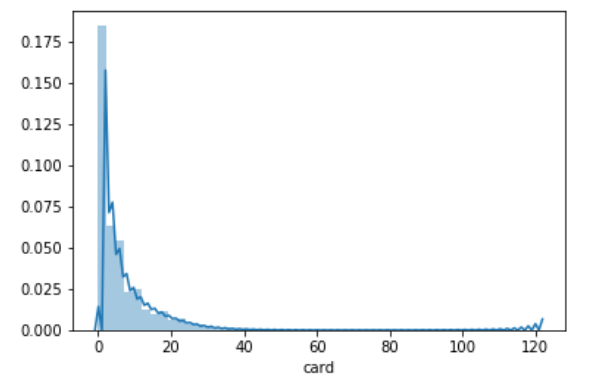
\includegraphics{11}
%     \captionof{figure}{User's 28-day bus card payment trip times and distribution map}
%     \label{fig:5.7}
% \end{minipage}
% \end{minipage}
    \item According to the data given in Appendix 1, we will take the given 28 days as the sample, take the number of trips 200 as the boundary, regard the data of more than 200 trips within 28 days as abnormal data, exclude this part of abnormal data, take the number of trips as the abscissa, and the proportion of this number of trips in the number of trips of all people as the ordinate. The histogram is shown in figures 5-5, 5-6 and 5-7. Among them, 5-5 is the proportion of travel times of the sum of the two methods for all people, 5-6 is the proportion of travel times of people using third-party payment platforms, and 5-7 is the proportion of travel times of people using bus cards.
\par
From the data in Figure~\ref{fig:5.5}, we can see that the vast majority of people travel 0-25 times in the sampling 28 days, and the peak can account for about 10\% of all people. From the data in Figure~\ref{fig:5.6}, we can see that the vast majority of people who use the third-party payment platform have traveled 0-20 times is the largest in the sampling 28 days.And the peak can account for about 15\% of all people. From the data in Figure~\ref{fig:5.7}, we can see that the vast majority of people who use bus cards have the largest number of trips ranging from 0 to 20 times in the sampling 28 days, and the peak can account for about 18\% of all people.
\par
It can be inferred from this that the general number of trips of people in the sampling 28 days is about 0-20. At the same time, among the people who travel 0-20 times, more people use bus cards than those who use third-party payment platforms, that is, among the people who travel at low frequency, more people choose bus cards.
% \begin{figure}[!ht]
%     \centering
%     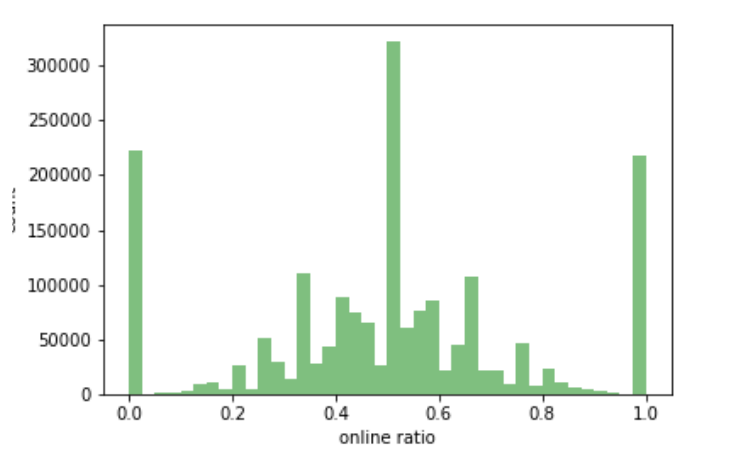
\includegraphics{12}
%     \caption{Distribution map of the ratio of the number of mobile payments to the total number of trips}
%     \label{fig:5.8}
% \end{figure}
    \item According to the data in Appendix 1, we separate the data of each person, divide the number of times each person uses the third-party mobile payment platform by the total number of times this person pays in two ways as the abscissa, and take the sum as the ordinate. The distribution diagram is shown in Figure~\ref{fig:5.8}.\\
\begin{minipage}{1.0\linewidth}
    \centering
    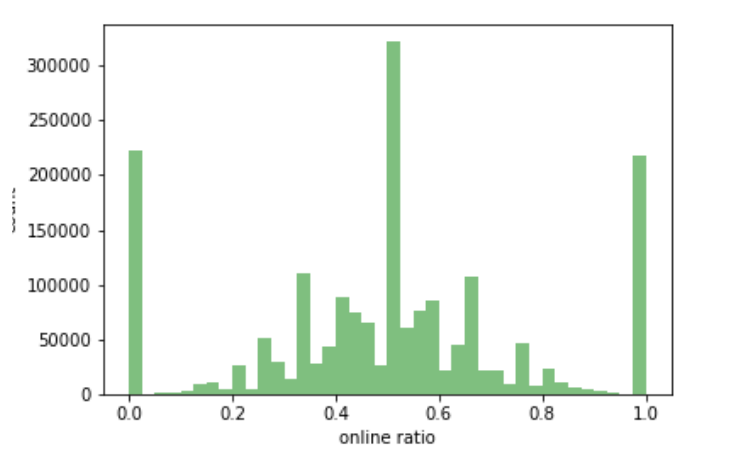
\includegraphics{12}
    \captionof{figure}{Distribution map of the ratio of the number of mobile payments to the total number of trips}
    \label{fig:5.8}
\end{minipage}
\par
We can get from the figure that the number of people with a ratio of 0.5 is the largest, that is, most people have the same probability of choosing a third-party mobile payment platform and bus card payment.
\par
We can get from the figure that the number of people with a ratio of 0.5 is the largest, that is, most people have the same probability of choosing a third-party mobile payment platform and bus card payment. At the same time, there are more people in 0 and 1, that is, more people choose bus card or third-party payment platform.
\par
The reason why so many people are distributed between 0 and 1 is that many people only record their one trip. When passengers choose a bus card for this trip, they will be distributed at the record point of 0. On the contrary, if they choose a third-party payment platform for payment this time, they will be recorded at the record point of 1.
\par
In order to reduce the impact of such one-time travelers on the results, we screened again and excluded all people with less than 50 trips within 28 days of the sample record. The distribution diagram is shown~in Figure~\ref{fig:5.9}.
\par
\begin{figure}[tp]
    \centering
    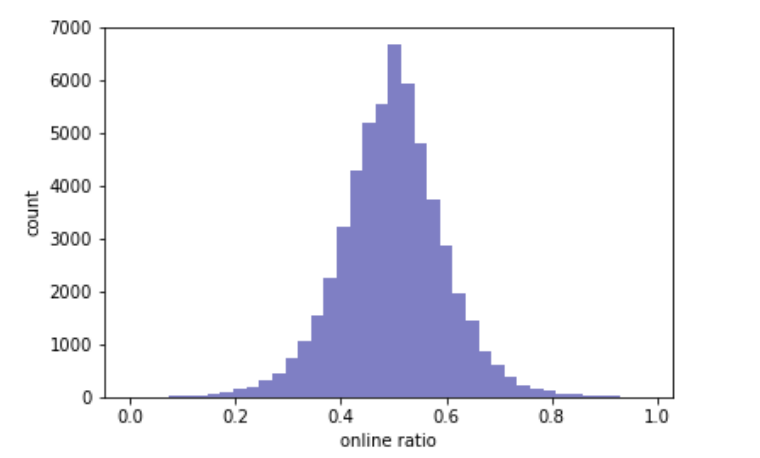
\includegraphics{13}
    \caption{Distribution of the ratio of the number of mobile payments to the total number of trips by high-frequency users}
    \label{fig:5.9}
\end{figure}
After removing the people with a small number of trips, we can see that the data distribution is obviously concentrated in the interval of 0.4-0.6, with a peak at 0.5, which basically shows a normal distribution, that is, most people choose third-party mobile payment platforms and public transportation. The probability of card trips is the same, or basically the same. From this, we can see that among the people who travel frequently, the vast majority of people will choose both bus cards and third-party mobile payment platforms to travel.
    \item According to the data given in Appendix 1, in order to intuitively see the aggregation degree of payment times using different payment methods at different times of each day, we set the abscissa to be each day when the data was collected (take February as an example), and the vertical The coordinates are set to 24 hours in a day, and the color depth is used to indicate the cumulative number of people who paid to get on the bus during this period. The darker the color, the higher the number of payments. The heat map generated based on the data is shown in Figure~\ref{fig:5.10} and Figure~\ref{fig:5.11}, where Figure~\ref{fig:5.10} represents the number of payments made using the bus card, and Figure~\ref{fig:5.11} represents the number of payments made using a third-party mobile payment platform.
\begin{figure}[!ht]
\centering
\begin{minipage}[c]{0.48\linewidth}
    \centering
    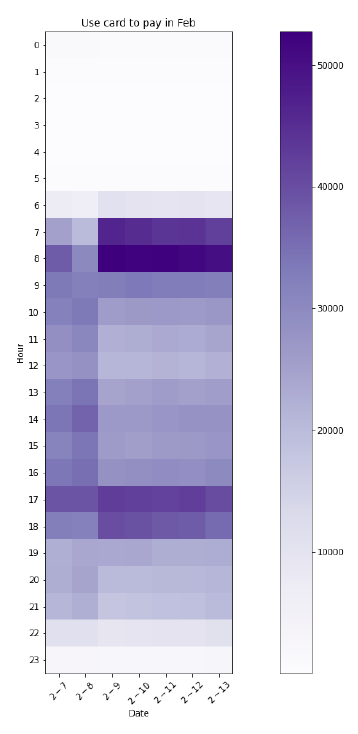
\includegraphics[scale=0.8]{14}
    \caption{Heat map of the number of bus card payments in February}
    \label{fig:5.10}
\end{minipage}
\quad
\begin{minipage}[c]{0.48\linewidth}
    \centering
    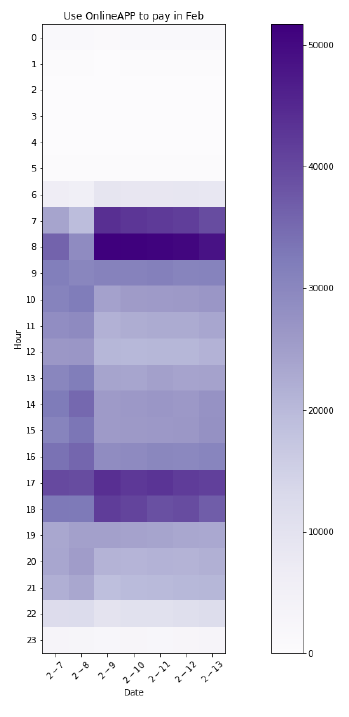
\includegraphics[scale=0.8]{15}
    \caption{Heatmap of Mobile Payments in February}
    \label{fig:5.11}
    \end{minipage}
\end{figure}
\end{enumerate}
\subsection{Summary of Data Analysis}
\indent{}According to the data form the attached file 1 and 2, we have more analysis about this.
\par
First of all, we can see that the time of sampling data is very scientific, and the months of 2, 5, 8 and 11 are selected that they avoid peak periods like summer and winter, and they also avoid holidays in the data collected during those months During the holidays, the seven days of universal significance were chosen. Seven days of data collection can also be seen in the Within a week, the change of payment times is conducive to reflect the reality.
\par
Secondly, before data analysis, we decided to remove abnormal data after the discussion. For example, the payment method is not the brush Card payment methods, and other methods that don't use either bus card payment or mobile payment, and swiping cards The number of unsuccessful payments, after deducting this part of abnormal data, we used software to analyze the data.
\par
Thirdly, we can know the peak of payment in a day by analyzing the change of payment times in 24 hours, and people's tendency to choose different payment methods. And then we looked at a week's worth of data from different months. How the number of payments changes and how people prefer the two payment methods from month to month. In the end, we classified different groups of people, and analyze the tendency of people with different travel times to choose the two payment methods.
\par
Finally, we draw some conclusions as follow:
\begin{enumerate}[label=\arabic*)]
    \item In one day, the morning peak occurs from 7 to 9 in the morning and the evening peak occurs from 17 to 19 in the evening. The number of payment times reaches the one-day peak, and the number of payment by bus card is more than that of mobile payment in the morning peak, while the situation is opposite in the evening peak.
    \item In a week, the data reflected that the number of payments made by bus card was slightly higher than that made by third-party payment platforms, and the difference between the two was the smallest on Sunday and the largest on Wednesday.
    \item In different months, as the months went by, the number of payments by bus card was slightly higher than the number of mobile payments, and gradually approached the number of payments by third-party mobile payment platforms, while both decreased.
    \item Low-frequency travelers and high-frequency travelers have roughly the same preference for payment by bus card and third-party mobile payment platform, that is, when faced with the choice of payment method, about half of them choose to pay by bus card, while the other half choose third-party mobile payment platform.
    \item For each passenger, excluding those with low travel times, the result of our data analysis is that the vast majority of people choose to use both payment methods at the same time, and there is no obvious preference for a certain payment method.
\end{enumerate}
Therefore, according to the data in Annex 1, we can draw preliminary conclusions about the payment characteristics of some people in the city above, and analyze the possible reasons for this.
\section{Model Estimating and Solving of Problem 2}
\subsection{Profit Model of Third-party Payment Platform}
With the continuous development of third-party payment platforms and the progress of mobile information technology, third-party payments have become an industry with good development prospects. The diversification of operation mode and profit mode makes it have strong market competitiveness. On normal third-party payment platforms, there are four profit models as follows:
\begin{enumerate}[label=\arabic*), itemindent=2\parindent, leftmargin=0pt, topsep=0pt, listparindent=\parindent, itemsep=1pt]
	\item poundage\par
Handling fee refers to the difference between the handling fee charged by the third-party payment platform and the procedure fee charged by the bank. Personal services provided by the third-party include transfer, payment, withdrawal, SMS security payment reminder and foreign currency payment, etc. The enterprise service is the commission of clearing transaction related services such as checking amount, checking account, closing payment and refund of money.
\par
The charge ratio ranges from 0.08\% to 1.25\%, and the charge ratio of transfer and withdrawal is 0.1\%. Different service types have different handling fees, and the proportion of handling fees charged for transactions of different amounts of the same service will also be different.
	\item advertising\par
As a high-frequency payment method, the third-party payment platform has a strong ability of publicity due to its convenient mobile client and corresponding Internet platform. Therefore, the third-party payment platform can charge merchants' advertising fees through advertising space as one of the profit channels.
	\item Interest income from deposited funds\par
The definition of precipitation funds is as follows: the pre-deposited currency payment funds actually received by the payment institution when handling the payment business entrusted by the customer.
\par
According to the relevant regulations in the "Administrative Measures for Customer Reserve Funds of Payment Institutions": the ratio of the risk reserve of the third-party payment platform shall not be lower than 1000 of the interest earned by the reserve fund in the bank account, and the highest profit of the third-party payment platform shall be It is 90 0 0 of the interest. According to the relevant regulations and the rules and regulations of the bank, part of the reserves can be deposited in the form approved by the People's Bank of China. The deposit forms are roughly: unit time deposit, demand deposit, agreement deposit and unit call deposit. Currently, demand deposits are used as the main deposit method, but the term shall not exceed three months. The agreed deposit rate of such deposits is roughly 400~500, and each deposit should also pay 0.7800 to the bank.
fee.
	\item service charge\par
The third-party payment platform can also provide payment solutions and various value-added services on the basis of providing a basic payment system. With the continuous expansion of the platform, urban life services are continuously combined with it, providing a variety of payment methods, such as electricity bills, water bills, mobile phone bills and other aspects. When the platform provides individuals or organizations with more convenient payment channels, it increases its competitiveness in the market, and at the same time, it charges part of the service fee as one of the platform's profit models. With the continuous improvement of technology and service capabilities, the platform has more competitiveness and attracts customers to expand its influence.
\end{enumerate}
\subsection{Expenditure Patterns of Third-party Payment Platforms}
\begin{enumerate}[label=\arabic*), itemindent=2\parindent, leftmargin=0pt, topsep=0pt, listparindent=\parindent, itemsep=1pt]
    \item advertising costs\par
The third-party payment platform cooperates with public transportation, and provides services such as daily recharge and use of transportation costs through the platform, adding new payment modes to facilitate more residents. In order to promote the new services of the third-party payment platform and make more passengers use the third-party payment platform for payment, it is necessary to carry out pre-publicity in newspapers, bus billboards, and station billboards to increase influence.
    \item access fee\par
The current interface access modes of third-party payment platforms mainly include computer website payment, mobile website payment, APP payment, etc. The payment interface rates of various third-party payment companies also tend to be the same. The general industry rate is around 0.6\%, entertainment and other virtual services, the rate is 1\%.
    \item fixed charges\par
The third-party payment platform requires fixed investment in personnel management, new project services, and bank docking during the operation stage. Such as the construction of infrastructure, the establishment and management of servers, and the negotiation of relevant agreements with banks for reserve funds. Therefore, it is necessary to carry out part of one-time fixed expenditures for infrastructure, etc., and part of continuous expenditures such as labor costs for personnel.
\end{enumerate}
\subsection{Profit model of third-party payment platform in public transportation system}
The public transportation system has clear economic characteristics, it is to meet the spatial displacement of people in the public area. Public transportation not only needs to meet the requirements of people's livelihood, but also needs to get remuneration from the service objects. When realizing its own economic benefits, it will also have an economic impact on the surrounding areas. At the same time, it has the characteristics of large flow, large amount, and inconvenient management. In addition, the operation of the public transportation system is greatly affected by external factors, policies and line planning.
will affect it.
\par
According to the above profit model and expenditure model combined with the environment and characteristics of the public transportation system, the exclusive model of its profit can be obtained:\\
% \begin{figure}[!ht]
% \centering
% 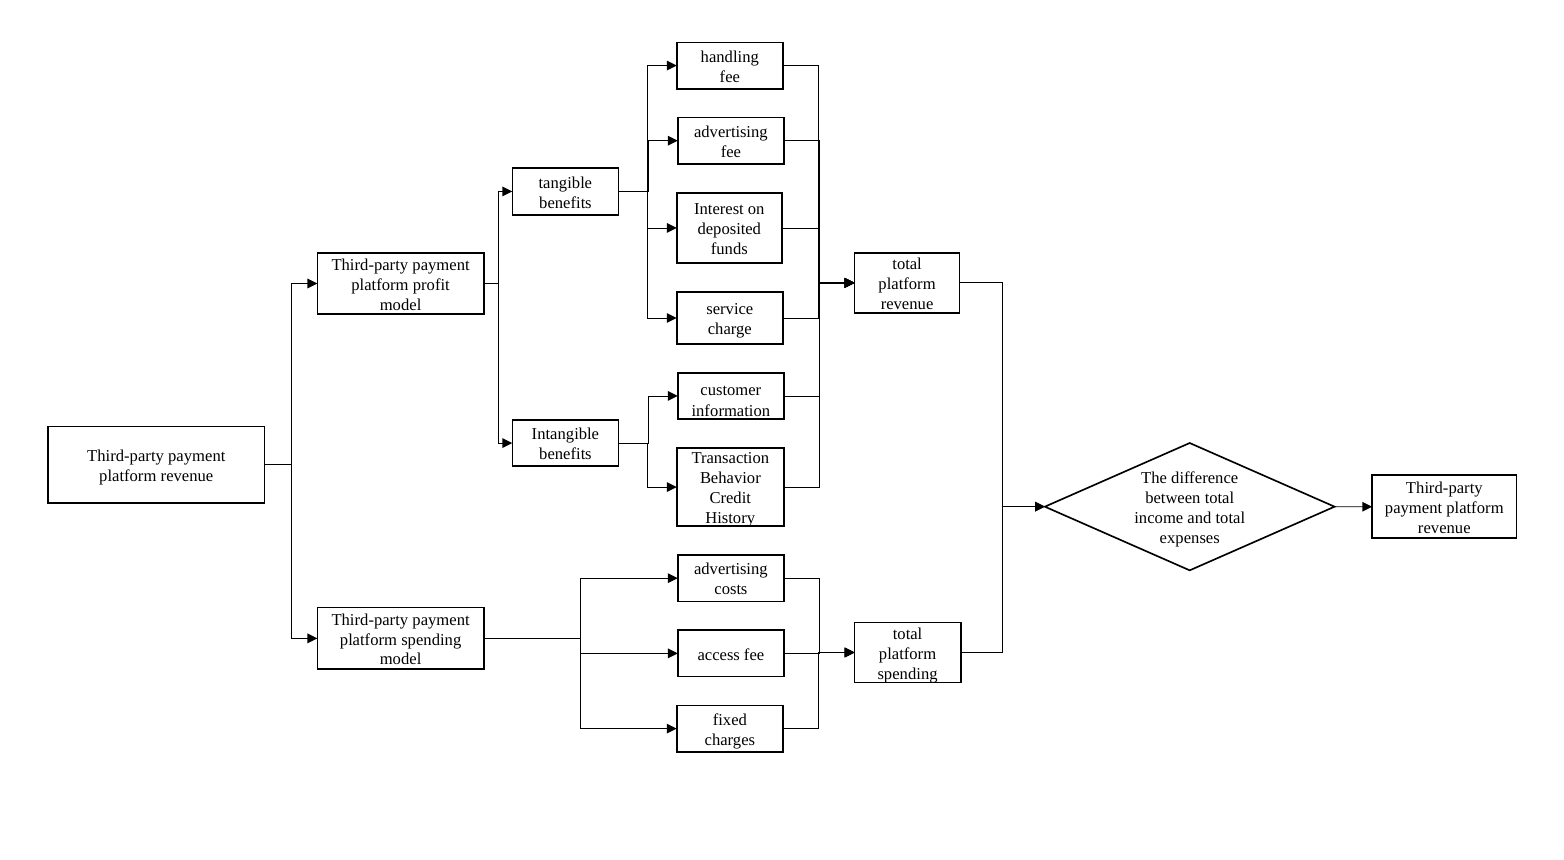
\includegraphics[scale=0.5]{16}
% \caption{Schematic diagram of profit model}
% \label{fig:5.12}
% \end{figure}
\begin{minipage}{1.0\linewidth}
\centering
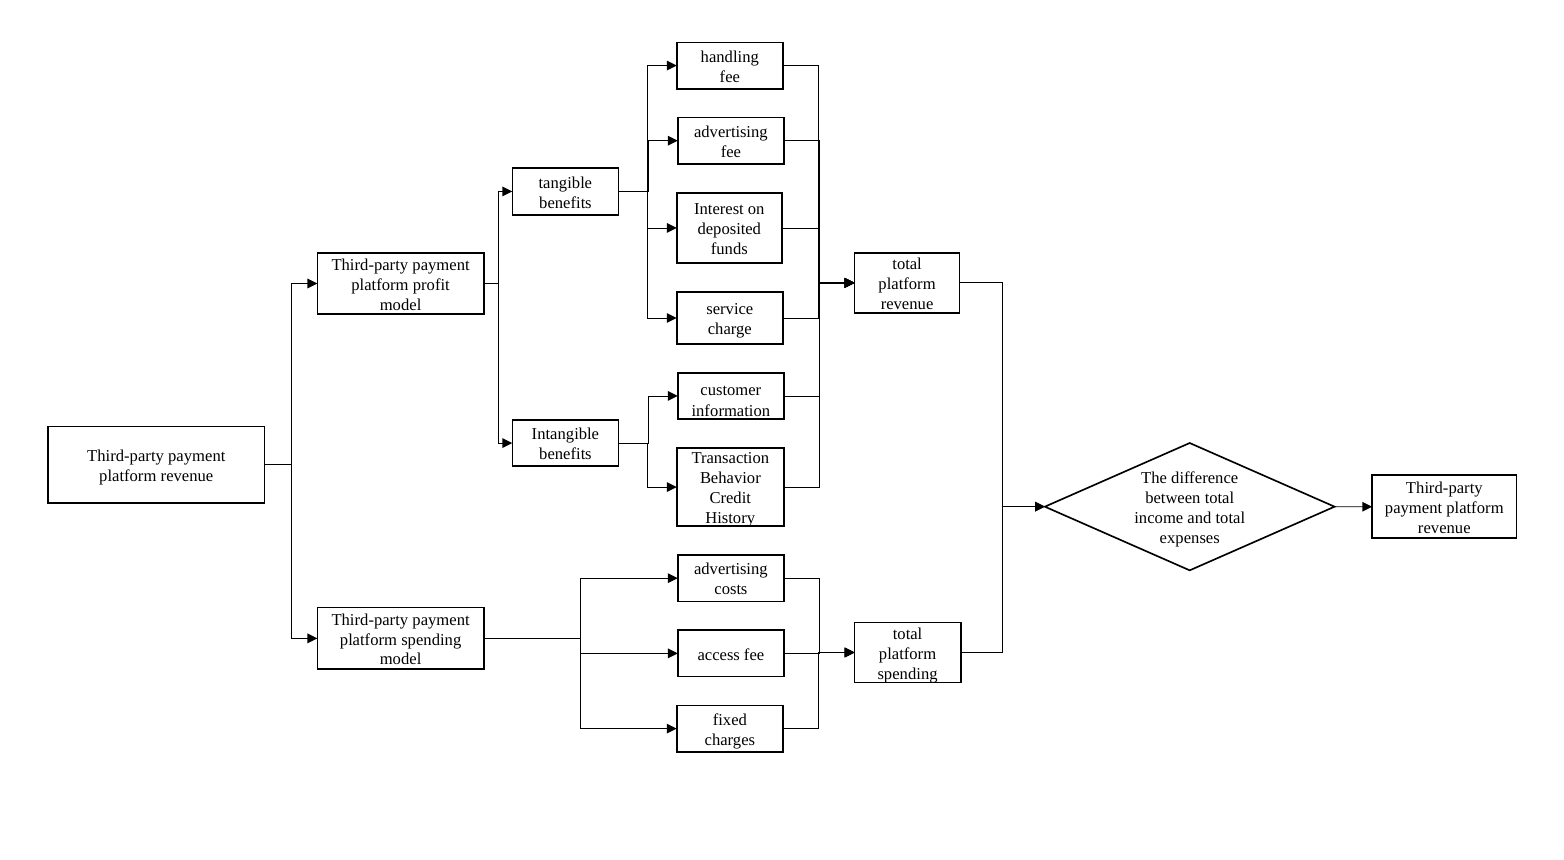
\includegraphics[scale=0.5]{16}
\captionof{figure}{Schematic diagram of profit model}
\label{fig:5.12}
\end{minipage}
\subsection{The Establishment of the Business Profit Mathematical Model of the Third-party Payment Platform}
According to the payment characteristics of public transportation combined with the profit model of the third-party payment platform, it is not difficult for us to draw the above-mentioned income-expense flow chart. Then there are:
\begin{equation}
W_0 = I_0 - O_0
\end{equation}
where $W_0$ is the profit of the model, $I_0$ is the total revenue of the model, and $O_0$ is the total expenditure of the model.
\par
From the above flow chart, it can be known that the mathematical expression of the total income $I_0$ is:
\begin{equation}
I_0 = I_1 + I_2 + I_3 + I_4
\end{equation}
Among them, $I_1$ is the interest income of precipitation funds, $I_2$ is the income of handling fees, $I_3$ is the income of service fees, and $I_4$ is the income of advertising fees.
\par
Mathematical calculation of interest $I_1$ of precipitation funds: The generation of interest of precipitation funds is a linear programming problem in dynamic changes, and its linear dynamic system formula is:
\begin{equation}
I_{n+1} = r(I_n+X_n+X_{n-1}+X_{n-2})
\end{equation}
Among them, $X_i$ is the total recharge amount of the $i$-th month, that is, the precipitation funds.($i=1,\dots,n$)
\par
The growth coefficient $r$ is determined:
\begin{equation}
r = a_1\bullet a_2\bullet(1-a_3)
\end{equation}
Among them, $a_1$ is the agreement deposit rate, $a_2$ is the maximum interest rate of the deposited funds, and $a_3$ is the handling fee agreed with the bank.
\par
According to the relevant agreement of the bank, demand deposit is the main deposit method, and its deposit period shall not exceed three months. Then there is the following calculation formula:
\begin{equation}
\begin{aligned}
&I_{n+1}=\left(r^{n}+r^{n-1}+r^{n-2}\right) \bullet X_{1}+\left(r^{n-1}+r^{n-2}+r^{n-3}\right) X_{2}+\dots \\
&+\left(r^{4}+r^{3}+r^{2}\right) X_{n-3}+\left(r^{3}+r^{2}+r\right) X_{n-2}+\left(r^{2}+r\right) X_{n-1}+r X_{n}
\end{aligned}
\end{equation}
Among them, $n\leq 1$, $X$ is the monthly recharge amount, that is, the deposited funds.($i=1,\dots,n$)
\par
Mathematical calculation of handling fee $I_2$: The charging ratio of handling fee is related to its recharge amount, then the mathematical formula about $I_2$ at this time is an interval function, and the selection of the interval point is related to the negotiated policy.
\begin{equation}
I_{2}= \begin{cases}r_{s} \bullet X_{s i} \bullet n & r_{s}=0.08\%\hspace{0.5
  em} X_{s i} \leq 100 \\ r_{s 1} \bullet X_{s i} \bullet n & r_{s}=0.1\% \quad X_{s i}>100\end{cases}
\end{equation}
Among them, $r_s$ and $r_{s1}$ are the charging ratio of the handling fee, $X_{si}$ is the single recharge amount in the i-th month, and $n$ is the number of people who recharged.
\par
Mathematical calculation of service fee $I_3$: The proportion of service fee charged is related to its amount, and has a lower limit of the fee and a limit of upper limits.
\begin{equation}
I_{3}=r_{f} \bullet X_{f i} \bullet n, \quad r_{f} \bullet X_{f i} \subseteq[0.5,10]
\end{equation}
In which $r_f$ is the charge ratio of service fee, $X_{fi}$ is the single amount in the $i$-month, the $r_f\bullet X_{fi}$ interval is $[0.5, 10]$, and $n$ is the number of recharge.
\par
The mathematical calculation of advertising cost 4I: the amount of advertising cost is related to the number of people. In the low interval, the advertising cost is constant, and in the high interval, the advertising cost is proportional to the number of people.
\begin{equation}
\begin{array}{ll}
I_{4}=A_{g} & n \leq N \\
I_{4}=A_{g}+n \bullet X_{g} & n>N
\end{array}
\end{equation}
Where $A_g$ is the one-off advertising fee paid in the low range, $X_g$ is the advertising fee earned on a single mobile platform in the high range, $n$ is the number of users of the platform, and $N$ is the threshold of the number of users.It can be seen from the above flow chart that the mathematical expression of total expenditure $O_0$ is
\begin{equation}
O_0 = O_1 + O_2 + O_3
\end{equation}
where $O_1$ is the advertising cost invested in the early stage, $O_2$ is the cost of mobile terminal access, and $O_4$ is the fixed expenditure.
\par
The calculation formula of the propaganda cost of the early advertising is:
\begin{equation}
O_1 = m\bullet X_c
\end{equation}
where $m$ is The Times of the early advertising investment and $X_c$ is the cost of a single publicity.
\par
The calculation formula of mobile terminal access charge $O_2$ is as follows:
\begin{equation}
O_2 = r_j\bullet X_j\bullet n
\end{equation}
Where $r_j$ is the charging rate of access fee, $X_j$ is the amount of the fee, and $n$ is the number of access.
\par
The mathematical calculation formula of fixed expenditure $O_3$ is as follows:
\begin{equation}
O_3 = A_j + A_x + n\bullet c\bullet X_r
\end{equation}
where $A_j$ is the input cost of infrastructure, $A_x$ is the fixed cost of new projects, $c$ is the number of employees, $X_r$ is the salary of employees, and $n$ is the number of working months.
\par
The integration of the above mathematical calculation formula of income and expenditure can be obtained:
\begin{equation}
\begin{gathered}
W_{0}=I_{0}-O_{0} \\
W_{0}=I_{1}+I_{2}+I_{3}+I_{4}-\left(O_{1}+O_{2}+O_{3}\right) \\
W_{0}=r\left(I_{n}+X_{n}+X_{n-1}+X_{n-2}\right)+r_{s} \bullet X_{s i} \bullet n+r_{f} \bullet X_{f i} \bullet n+A_{g}+n \bullet X_{g}- \\
\left(m \bullet X_{c}+r_{j} \bullet X_{j} \bullet n+A_{j}+A_{x}+n \bullet c \bullet X_{r}\right)
\end{gathered}
\end{equation}
including:
\begin{equation}
\left\{\begin{array}{l}
n \geq 1, i=1 \ldots \ldots n \\
r_{s}=0.08 \%, X_{s i} \leq 100 \\
r_{s}=0.1 \%, X_{s i}>100 \\
r_{f} \bullet X_{f i} \subseteq[0.5,10] \\
n \leq N, X_{g}=0 \\
r \geq 0, X \geq 0, r_{s} \geq 0, X_{s i} \geq 0, r_{f} \geq 0, X_{f i} \geq 0, A_{j} \geq 0, A_{x} \geq 0
\end{array}\right.
\end{equation}
\subsection{Quantitative analysis of profit mathematical model model}
\subsubsection{Quantitative analysis of total revenue $I_0$}
\begin{enumerate}[label=\arabic*)]
    \item Quantitative analysis and calculation of precipitation fund $I_1$ determination of growth coefficient $r$
\begin{equation}
r=a_1\bullet a_2\bullet (1-a_3)
\end{equation}
where $a_{1}$ is the agreement deposit rate, $a_2$ is the highest acquisition rate of precipitation fund interest, and $a_3$ is the commission fee agreed with the bank. Then
\begin{equation}
\begin{cases}
a_{1} = 4.5\% \\
a_2 = 90\% \\
a_3 = 0.78\%
\end{cases}
\end{equation}
Substitution: $r=0.045 \bullet 0.9 \bullet(1-0.0078)=0.0401841 \approx 0.04$
\par
$X_i$ is the total recharge amount of month $i$, i.e. precipitation fund ($i=1, 2,\dots, n$), then $X_i$ is the independent variable:
\begin{equation}
I_{n+1}=r\left(I_{n}+X_{n}+X_{n-1}+X_{n-2}\right)=0.04\left(I_{n}+X_{n}+X_{n-1}+X_{n-2}\right)
\end{equation}
    \item Quantitative analysis and calculation of procedure cost $I_2$: The calculation formula of procedure cost is as follows:
\begin{equation}
I_2=r_s\bullet X_{xi}\bullet n
\end{equation}
this function is an interval function, and the interval point is determined by the charging system to be 100, i.e. the discontinuity point when $X_{si}=100$:
\begin{equation}
\left\{\begin{array}{l}
r_{\mathrm{s}}=0.08 \%, X_{\mathrm{si}} \leq 100 \\
r_{\mathrm{s}}=0.1 \%, X_{\mathrm{si}}>100
\end{array}\right.
\end{equation}
Wheres $X_i$ is the single recharge amount in $i$-month  and $n$ is the number of recharge people, which constitute the independent variables of this function.
    \item Quantitative analysis and calculation of service fee $I_3$: The calculation formula of service fee is as follows:
\begin{equation}
I_3=r_f\bullet X_{fi}\bullet n
\end{equation}
According to relevant payment regulations:
\begin{equation}
r_f=0.1\%
\end{equation}
where $X-fi$ is the single amount in the $i$-th month and $n$ is the number of recharge, both of which are independent variables of the function.But due to the restrictions of relevant regulations, $I_3$ had a corresponding value range $r_f\bullet X_{fi}\in [0.5, 10]$, i.e. and it was proved that:
\begin{equation}
\left\{\begin{array}{l}
X_{f i \min }=\frac{0.5}{0.1 \%}=500 \\
X_{f i \max }=\frac{10}{0.1 \%}=10000
\end{array}\right.
\end{equation}
The piecewise function is valid:
\begin{equation}
\left\{\begin{array}{l}
I_{3}=0, X_{f i}<500 \\
I_{3}=r_{f} \bullet X_{f i}, 500 \leq X_{f i} \leq 10000 \\
I_{3}=10, X_{f i}>10000
\end{array}\right.
\end{equation}
    \item Quantitative analysis calculation of advertising cost $I_4$:
\begin{equation}
\begin{cases}I_{4}=A_{g} & n \leq N \\ I_{4}=A_{g}+n \bullet X_{g} & n>N\end{cases}
\end{equation}
Determination of threshold $n$:There are two influencing factors that determine $n$: on the one hand, the number of users using mobile platforms $n$, and on the other hand, the implicit function of influence $f(n)$.
The function of the threshold $n$ is determined as follows :
\begin{equation}
N=\phi\bullet n\bullet f(n) + \gamma
\end{equation}
where $n$ is the number of mobile devices in the third-party payment platform, $\phi$ is the prediction coefficient of the number of users, $f(n)$ is the implicit function of influence, and $\pi$ is the error value.
\end{enumerate}
\subsubsection{Quantitative analysis of total expenditure $O_{1}$}
\begin{enumerate}[label=\arabic*)]
    \item Quantitative analysis calculation of $O_1$ advertising and publicity expenses in the early stage:
\begin{equation}
O_1=m\bullet X_c
\end{equation}
where $m$ is the number of times invested in publicity in the early stage and $X_c$ is the cost of a single publicity $m$ and $X_c$ are independent variables of the function and are related to the agreements signed by the third-party payment platform and strategic objectives. According to the analysis data and collection of relevant information, $m$ and $X_c$ are taken as the arithmetic average value of each type:
\begin{equation}
\left\{\begin{array}{l}
m=\dfrac{m_{1}+m_{2}+m_{3}+\ldots .+m_{n}}{n}=\dfrac{\sum_{i=1}^{n} m_{i}}{n} \\[2em]
X_{c}=\dfrac{X_{c 1}+X_{c 2}+X_{c 3}+\ldots .+X_{c n}}{n}=\dfrac{\sum_{i=1}^{n} X_{c i}}{n}
\end{array}\right.
\end{equation}
    \item Quantitative analysis and calculation of mobile terminal access charge $O_2$
\begin{equation}
O_2 = r_j\bullet X_j\bullet n
\end{equation}
where the charging ratio of access charge $r_j$ and the amount of charge $X_j$ are the main influencing variables.According to third-party industry payment guidelines:\\
\begin{minipage}{1.0\linewidth}
\captionof{table}{Table of Payment Guidelines for Third-Party Industries}
\begin{tblr}{
      width=\linewidth,
      colspec={X[c]X[c]X[-1, c]X[-1, c]X[-1,c]},
      hline{1, Z} = {2pt, solid},
      hline{2} = {solid}
    }
    Product Name  & Application Scenario(yuan) &  Access Fee & Rate & Margin(yuan) \\ 
AAP Payment & Mobile application & 0  &  General industry: 0.6\% & 0  \\
Mobile website payment & Mobile web page  & 0 &  General industry:0.6\% & 0\\ 
computer website pay & PC web page & 0 & General Industry: 0.6\% & 0\\ 
Pay in person & scan code & 0 & General industry: 0.6\% & 0\\
Transfer to account  & Enterprise payment & 0  & free & 0 \\ 
Alipay batch payment & Enterprise payment & 0  & single payment rate: 0.5\% & 0
\end{tblr}
\end{minipage}\\[1em]
According to the table: The charging ratio of access fee
\begin{equation}
r_j = 0.6\%
\end{equation}
    \item Quantitative analysis and calculation of fixed expenditure $O_3$
\begin{equation}
O_3 = A_j+A_x+n\bullet c\bullet X_r
\end{equation}
where $A_j$ is the input cost of infrastructure, $A_x$ is the fixed cost of new project, $c$ is the number of employees, $X_r$ is the employee salary, and $n$ is the number of working months. $A_j$ and $A_x$ are determined values. $c, X_r$ and $n$ are all variables and are related to the actual situation.

\end{enumerate}
\subsubsection{Quantitative Analysis of Total Profit $W_0$}
\begin{equation}
W_0=I_o - O_0
\end{equation}
\begin{equation}
W_0=I_1+I_{2}+I_3+I_4-(O_0+O_1+O_2)
\end{equation}
Substitute the values after quantitative analysis into:
\begin{equation}
\begin{gathered}
W_{0}=r\left(I_{n}+X_{n}+X_{n-1}+X_{n-2}\right)+r_{s} \bullet X_{s i} \bullet n+r_{f} \bullet X_{f i} \bullet n+A_{g}+n \bullet X_{g}- \\
\left(m \bullet X_{c}+r_{j} \bullet X_{j} \bullet n+A_{j}+A_{x}+n \bullet c \bullet X_{r}\right)
\end{gathered}
\end{equation}
According to the classification of different constraints, we can obtain the following expressions and constraints:
\ding{172}
\begin{equation}
\begin{aligned}
&W_{0}=0.04\left(I_{n}+X_{n}+X_{n-1}+X_{n-2}\right)+0.08 \% \bullet X_{\mathrm{si}} \bullet n+0.1 \% \bullet X_{f i} \bullet n+A_{g}+n \bullet X_{g} \\
&-\left(\frac{\sum_{i=1}^{n} m_{i}}{n} \bullet \frac{\sum_{i=}^{n} X_{c i}}{n}+0.6 \% \bullet X_{j} \bullet n+A_{j}+A_{x}+n \bullet c \bullet X_{r}\right)\\
\end{aligned}
\end{equation}
\begin{equation}
\left\{\begin{array}{l}
X_{s i} \leq 100 \\
500 \leq X_{f i} \leq 10000 \\
n>N \\
X \geq 0, r_{s} \geq 0, A_{j} \geq 0, A_{x} \geq 0
\end{array}\right.
\end{equation}
\ding{173}
\begin{equation}
\begin{aligned}
&W_{0}=0.04\left(I_{n}+X_{n}+X_{n-1}+X_{n-2}\right)+0.1 \% \bullet X_{s i} \bullet n+0.1 \% \bullet X_{f i} \bullet n+A_{g}+n \bullet X_{g} \\
&-\left(\dfrac{\sum_{i=1}^{n} m_{i}}{n} \cdot \dfrac{\sum_{i=}^{n} X_{c i}}{n}+0.6 \% \cdot X_{j} \cdot n+A_{j}+A_{x}+n \bullet c \bullet X_{r}\right) \\
&\hspace{10em}\left\{\begin{array}{l}
X_{s i}>100 \\
500 \leq X_{f i} \leq 10000 \\
n>N \\
X \geq 0, r_{s} \geq 0, A_{j} \geq 0, A_{x} \geq 0
\end{array}\right.
\end{aligned}
\end{equation}
\ding{174}
\begin{equation}
\begin{aligned}
W_{0}&=0.04\left(I_{n}+X_{n}+X_{n-1}+X_{n-2}\right)+0.08 \% \bullet X_{s i} \bullet n+0+A_{g}+n \bullet X_{g} \\
&-\left(\dfrac{\sum_{i=1}^{n} m_{i}}{n} \cdot \dfrac{\sum_{i=}^{n} X_{c i}}{n}+0.6 \% \cdot X_{j} \bullet n+A_{j}+A_{x}+n \bullet c \bullet X_{r}\right) \\
&\hspace{10em}\left\{\begin{array}{l}
X_{s i} \leq 100 \\
X_{f i}<500 \\
n>N \\
X \geq 0, r_{s} \geq 0, A_{j} \geq 0, A_{x} \geq 0
\end{array}\right.
\end{aligned}
\end{equation}
\ding{175}
\begin{equation}
\begin{aligned}
W_{0}&=0.04\left(I_{n}+X_{n}+X_{n-1}+X_{n-2}\right)+0.1 \% \bullet X_{s i} \bullet n+0+A_{g}+n \bullet X_{g} \\
&-\left(\dfrac{\sum_{i=1}^{n} m_{i}}{n} \cdot \dfrac{\sum_{i=}^{n} X_{c i}}{n}+0.6\% \cdot X_{j} \bullet n+A_{j}+A_{x}+n \bullet c \bullet X_{r}\right) \\
&\hspace{10em}\left\{\begin{array}{l}
X_{s i} \leq 100 \\
X_{f i}<500 \\
n>N \\
X \geq 0, r_{s} \geq 0, A_{j} \geq 0, A_{x} \geq 0
\end{array}\right.
\end{aligned}
\end{equation}
\ding{176}
\begin{equation}
\begin{aligned}
W_{0}&=0.04\left(I_{n}+X_{n}+X_{n-1}+X_{n-2}\right)+0.1 \% \bullet X_{s i} \bullet n+0+A_{g}+n \bullet X_{g} \\
&-\left(\dfrac{\sum_{i=1}^{n} m_{i}}{n} \cdot \dfrac{\sum_{i=}^{n} X_{c i}}{n}+0.6\% \cdot X_{j} \bullet n+A_{j}+A_{x}+n \bullet c \bullet X_{r}\right) \\
&\hspace{10em}\left\{\begin{array}{l}
X_{s i} \leq 100 \\
X_{f i}>10000 \\
n>N \\
X \geq 0, r_{s} \geq 0, A_{j} \geq 0, A_{x} \geq 0
\end{array}\right.
\end{aligned}
\end{equation}
\ding{177}
\begin{equation}
\begin{aligned}
W_{0}&=0.04\left(I_{n}+X_{n}+X_{n-1}+X_{n-2}\right)+0.1 \% \bullet X_{s i} \bullet n+0+A_{g}+n \bullet X_{g} \\
&-\left(\dfrac{\sum_{i=1}^{n} m_{i}}{n} \cdot \dfrac{\sum_{i=}^{n} X_{c i}}{n}+0.6\% \cdot X_{j} \bullet n+A_{j}+A_{x}+n \bullet c \bullet X_{r}\right) \\
&\hspace{10em}\left\{\begin{array}{l}
X_{s i} \leq 100 \\
X_{f i}>10000 \\
n>N \\
X \geq 0, r_{s} \geq 0, A_{j} \geq 0, A_{x} \geq 0
\end{array}\right.
\end{aligned}
\end{equation}
\ding{178}
\begin{equation}
\begin{aligned}
W_{0}&=0.04\left(I_{n}+X_{n}+X_{n-1}+X_{n-2}\right)+0.1 \% \bullet X_{s i} \bullet n+0+A_{g}+n \bullet X_{g} \\
&-\left(\dfrac{\sum_{i=1}^{n} m_{i}}{n} \cdot \dfrac{\sum_{i=}^{n} X_{c i}}{n}+0.6\% \cdot X_{j} \bullet n+A_{j}+A_{x}+n \bullet c \bullet X_{r}\right) \\
&\hspace{10em}\left\{\begin{array}{l}
X_{s i} \leq 100 \\
X_{f i}>10000 \\
n>N \\
X \geq 0, r_{s} \geq 0, A_{j} \geq 0, A_{x} \geq 0
\end{array}\right.
\end{aligned}
\end{equation}
\ding{179}
\begin{equation}
\begin{aligned}
W_{0}&=0.04\left(I_{n}+X_{n}+X_{n-1}+X_{n-2}\right)+0.1 \% \bullet X_{s i} \bullet n+0+A_{g}+n \bullet X_{g} \\
&-\left(\dfrac{\sum_{i=1}^{n} m_{i}}{n} \cdot \dfrac{\sum_{i=}^{n} X_{c i}}{n}+0.6\% \cdot X_{j} \bullet n+A_{j}+A_{x}+n \bullet c \bullet X_{r}\right) \\
&\hspace{10em}\left\{\begin{array}{l}
X_{s i} \leq 100 \\
X_{f i}>10000 \\
n>N \\
X \geq 0, r_{s} \geq 0, A_{j} \geq 0, A_{x} \geq 0
\end{array}\right.
\end{aligned}
\end{equation}
\ding{180}
\begin{equation}
\begin{aligned}
W_{0}&=0.04\left(I_{n}+X_{n}+X_{n-1}+X_{n-2}\right)+0.1 \% \bullet X_{s i} \bullet n+0+A_{g}+n \bullet X_{g} \\
&-\left(\dfrac{\sum_{i=1}^{n} m_{i}}{n} \cdot \dfrac{\sum_{i=}^{n} X_{c i}}{n}+0.6\% \cdot X_{j} \bullet n+A_{j}+A_{x}+n \bullet c \bullet X_{r}\right) \\
&\hspace{10em}\left\{\begin{array}{l}
X_{s i} \leq 100 \\
X_{f i}>10000 \\
n>N \\
X \geq 0, r_{s} \geq 0, A_{j} \geq 0, A_{x} \geq 0
\end{array}\right.
\end{aligned}
\end{equation}
\ding{181}
\begin{equation}
\begin{aligned}
W_{0}&=0.04\left(I_{n}+X_{n}+X_{n-1}+X_{n-2}\right)+0.1 \% \bullet X_{s i} \bullet n+0+A_{g}+n \bullet X_{g} \\
&-\left(\dfrac{\sum_{i=1}^{n} m_{i}}{n} \cdot \dfrac{\sum_{i=}^{n} X_{c i}}{n}+0.6\% \cdot X_{j} \bullet n+A_{j}+A_{x}+n \bullet c \bullet X_{r}\right) \\
&\hspace{10em}\left\{\begin{array}{l}
X_{s i} \leq 100 \\
X_{f i}>10000 \\
n>N \\
X \geq 0, r_{s} \geq 0, A_{j} \geq 0, A_{x} \geq 0
\end{array}\right.
\end{aligned}
\end{equation}
\subsubsection{Exact Calculation of Mathematical Model}
Take Model 9 as an example for calculation: Due to the imperfections of known data, after quantitative analysis of existing coefficients, the unknown independent variables are predicted and analyzed according to the basic data provided in the attachment.At the same time, combined with relevant public transport data, mathematical induction method is used to make reasonable inference, so as to obtain the following data:
Table model value table just following.\\[1em]
\begin{tblr}{
      width=\linewidth,
      colspec={X[c]X[c]*{11}{X[-1, c]}},
      hline{1, Z} = {2pt, solid},
      hline{2} = {solid}
    }
    $I_n$ & $X_n$ & $X_{n-1}$ & $X_{si}$ & $X_{fi}$ & $A_g$ & $X_g$ & $m_j$ & $X_{ci}$ & $X_j$ & $n$\\
    $8.1x10^6$ & $6.6x10^{7}$ & $6.6x10^{7}$ & 20 & 20& $1x10^{10}$ & 15 & 3 &$1x10^6$ & 20 & $3.3x10^{6}$
\end{tblr}\\[1em]
Then substitute into the formula of the mathematical model for calculation and obtain:
\begin{equation}
W_{0}=I_{0}-O_{0}=(810+5.28+100+0-600-39.6-85) \times 10^{4}=1906800
\end{equation}
To sum up, under the normal profit model, based on the existing attachment data of the third-party payment platform profit in roughly 61.910 x yuan, belong to the high profit of third-party payment platform.
\subsubsection{Analysis of Profit Mathematical Model of Third-party Payment Platform}
The composition of profit model is based on the meaning of "profit", that is, "the value of profit is the difference between total revenue and total expenditure".The mathematical formula is $W_0=I_0-O_0$ ($W_0$ is the profit of the model, $I_0$ is the total income of the model, and $O_0$ is the total expenditure of the model).In this problem, it is necessary to first define the components of income and expenditure, and then establish corresponding mathematical models according to the different situations of each part.Because of the economic characteristics of third-party payment platforms, their income is characterized by "charging corresponding fees in proportion", two aspects of piecewise function and linear programming are considered in the establishment of mathematical models.For the determination of the interval points of key variables, that is, the threshold value, the complex function or even the implicit function is established to solve, in order to get a more reasonable segmentation scheme and interval.In the process of establishing the model, Many of the scale factors Ri are selected according to existing regulations and try to match the real data.In the final model, there are still parts that need to be improved, for example, when determining the advertising cost $I_4$, its threshold $N=\phi\bullet n\bullet f(n)+\sigma$, in which the implicit function of influence $f(n)$ and error correction $\sigma$ need further verification and calculation, so as to obtain more accurate quantitative calculation results.
\end{document}
%%% Local Variables:
%%% mode: latex
%%% TeX-master: "../mcmpaper"
%%% End:
